\chapter{Introduction}

\epigraph{Let us, then, omit the conjectures of men who know not what they say,
    when they speak of the nature and origin of the human race... They are
    deceived, too, by those highly mendacious documents which profess to give
    the history of many thousand years, though, reckoning by the sacred
    writings, we find that not 6000 years have yet passed.}{St. Augustine, c.
    397 CE}


\section{The problem}

% Make this more of a lead-in to the rtmd, NDI and dual-system learning

Various human efforts, over the course of history, have drastically improved the
comprehensibility of our world. Along with this, the scope of our power to alter
our world has increased dramatically. Unfortunately, these alterations are not
always for the better, as is the case with global climate change. There is broad
agreement that anthropogenic (human caused) climate change is currently and will
continue to have negative consequences on both human and other forms of life on
our planet (for example, about 97\% of publishing climate scientists hold this
view). Certainly, some may say, the planet will endure. But, it seems wise
to proceed with some concern towards ensuring the survival of those organisms
and species we hold most dear.

While humans continue to increase our understanding of the world, issues like
climate change appear to be a bit beyond what is readily comprehended by
non-specialists. In particular, there seems to be a trouble with the
comprehension and acceptance of climate change in America. While much of the
developed world accepts anthropogenic climate change as a reality, as of January
2010 only 57\% of individuals surveyed in the United States think global warming
is happening at all. When asked to assume that global warming \emph{is}
happening, only 47\% of the same group of respondants indicated that they
thought it was ``caused mostly by human activities'' \cite<Q47 and Q50
in>{leiserowitz_climate_2010}.  Presumably, the number of Americans accepting
anthropogenic climate change is somewhat less than this figure. Thus, if we want
to do something about this issue in the context of a democratic society, the
first step is getting a reasonable majority of people to accept that there at
least \emph{may} be a problem \cite{prochaska_toward_1986}.  
% Note - Canny thinks the TTM cited here is not terribly relevant
Thus, the overarching question, ``How can ideas from cognitive science help us
improve climate change education?''

Certainly, the scope of climate change cognition is far too broad for a research
project of only a few semesters. As such, I will focus on a handful of issues
that are of interest from the point of view of a cognitive theory of learning.
Simultaneously, we maintain an educational point of view that entails a focus on
variables that we might control. I assume a pragmatic sense of ``poor'' and
``good'' cognition regarding climate change and related conceptual domains. The
goal will be to obtain an understanding that allows us to shift individuals from
the former to the latter. Roughly speaking, ``good'' cognition would allow
people to reason more accurately and be more robust to the problematic
arguments they are likely to encounter in our current political landscape.
Specific features of such cognition might include:

\begin{enumerate}
\item Reasoning with \emph{evidence}. In particular, the use of specific,
quantitative information (as discussed in section~\ref{sec:ndi} below).
\item Fluency with models used to explain and predict climate change.
\item Skeptical evaluation of evidence offered by others.
\item Ability to connect one's personal values and beliefs to policy
preferences.
\end{enumerate}

In an ideal world, the structure of this thesis would harken back to early
psychophysical research. There are a number of factors that we are certain will
induce surprise, acceptance of novel ideas and other forms of learning. A
lovely question could take the form of ``How many units of surprise yield so and
so units of attitudinal shift?'' or ``When matched for identical amounts of
cognition, what is the relative effect of numerically-grounded evidence vs.\
emotionally charged evidence?'' As is plain to see, such precision is well
beyond the current state of the art. Thus, I will focus primarily on categorical
differences between educational interventions and participants memories and
explanations. Below, I lay out a number of issues that figure heavily into the
selection of these categories.

\section{Reinforced Theistic Manifest Destiny theory}

%% Problematically, Al Gore also talks a lot about melting ice - arguing against
%% the bulk of our pro-GW items!

\citeA{ranney_why_inpress} observe that in addition to America's disparity
with peer nations in accepting global warming, Americans are also appreciably
lower in their acceptance of Darwinian evolution. Indeed, the United States
ranks 33rd of 34 peer nations in acceptance of evolution, putting us
squarely between Cypress and Turkey. The ``received view'' is that Americans are
particularly fundamentalist in their acceptance of biblical creation\footnote{I
will focus primarily on the Christian faith, as it is the dominant religion in
the U.S.\ and peer nations of interest. 84\% of Americans practice some form of
Christianity, with Judaism and Islam as the second and third most common at
1.9\% and 1.6\% respectively \cite{wolfram_alpha_faith}.}, 
necessitating the rejection of evolutionary ideas. But, this notion fails to
address the similar pattern observed with acceptance of climate change. In
addition, many of the afore-mentioned peer nations also exhibit high adherence
to Christian faiths.  Likewise, it is not clear that America is sufficiently
more fundamentalist than peer nations to explain all the important variance in
our acceptance of these ideas. 

\begin{figure}[h]
\centering
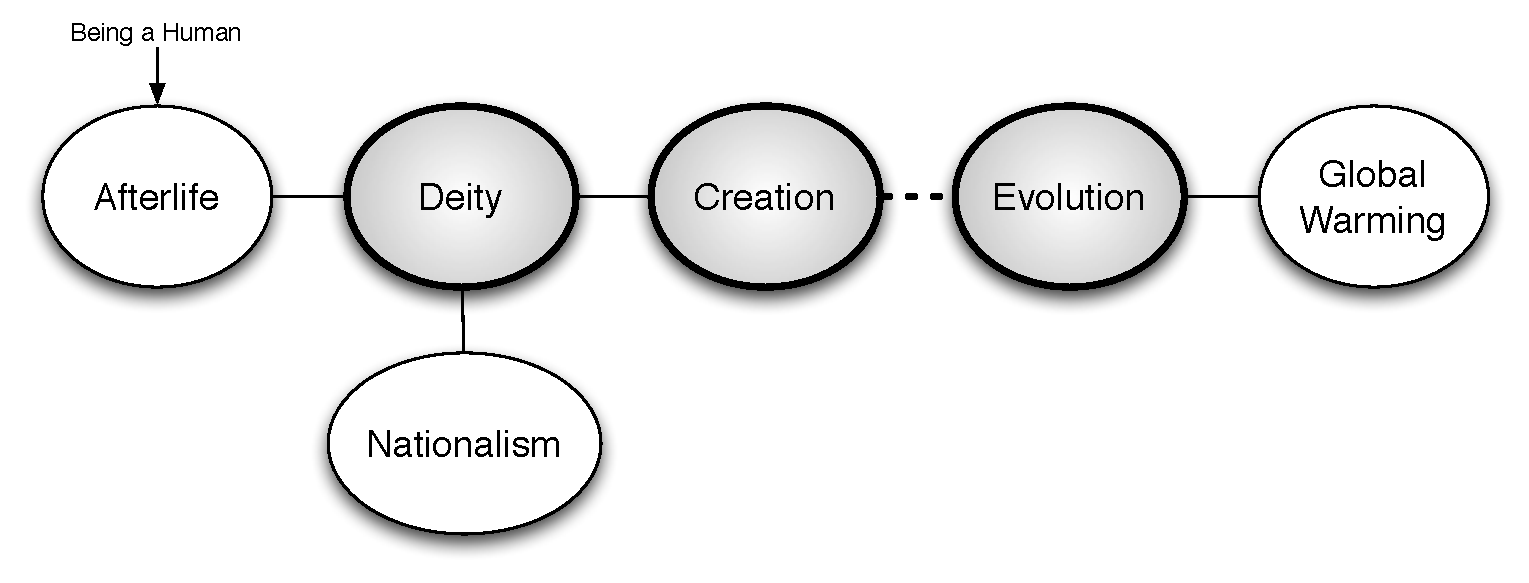
\includegraphics[width=\textwidth]{rtmd.pdf}
\caption{Ranney's RTMD model. The ``received view'' is emphasized, with
a negative relationship between belief in creation and acceptance of evolution
represented by the dashed line. Solid lines express positive relationships
between these and a network of related attitudes. A causal point of entry is
expressed for ``being a human,'' fearing death and thus, desiring an afterlife.}
\label{fig:rtmd} 
\end{figure}

The central insight of \citeA{ranney_accepting_2011} is that what sets the
United States apart from the rest of the world is the relative success it has
experienced over the previous century, called by some ``The American Century.''
Our war efforts have been (or at least seem) enormously successful, our economy
is far larger than any other economy in the world, we are successful in the
Olympics and so on. This leads to a
feeling that ``God is on our side,'' or in other words, it reinforces notions of
manifest destiny via quasi-religious sentiment.


Another general problem identified within RTMD is the fact that individuals
often reject scientific ideas when they are in conflict with their other
attitudes and beliefs. It's as if we are endowed with something of a conceptual
immune system, % Maybe elaborate more in thesis?
comprising religious and nationalistic beliefs in some, and more
scientifically grounded beliefs in others.  But note, there is a sharp distinction between
the kinds of ``emotional responses'' that might be experienced between climate
change and evolution. Specifically, climate change is something that
involves the ethical status of actions that we do every day, both individually
and as a society. Evolution, on the other hand, tends to incohere with
personally held religious beliefs, most directly divine creation, but then by
extension, deity and afterlife.

As an interesting side-note, both evolution and climate science require vastly
larger views of time as compared to many other sciences. The longest sample of
atmospheric greenhouse gasses and global temperature goes back an impressive
800,000 years.  Impressive, that is, until you consider that most major phyla
emerged around 530 million years ago (and have thus been influencing the climate
since that time).

% An interesting point of comparison would be Plate Tectonics (which apparently
% is also quite controversial in the south

RTMD doesn't disagree with other explanations, such as an analysis of
individuals into democrats and republicans. Rather, it provides a more specific
set of proximal relationships between concepts. According to the theory, for
example, acceptance of evolution should have \emph{more} predictive value for
one's global warming acceptance as compared to, say, acceptance of a deity.
Additionally, these relationships may predict related changes we might see as we
modulate individual's attitudes.


% Perhaps mention the inclusion of notions of consumerism?

\section{Reasoning with Numbers \label{sec:ndi}}

% It would probably make sense to highlight a more social psych citation here,
% as it would be more germane to climate change. Perhaps even one of the more
% recent climate change polarization articles?

NDI procedures \cite<introduced by>{ranney_numerically_2001_fixed} provide an
approach to changing conceptions, attitudes and even behaviors with quite
minimalist interventions (e.g., providing estimators with a single, critical,
highly germane, feedback statistic, \citeNP<cf.>{rinne_estimation_2006}).  The
education and social psychology literature provide multiple examples of failures
to elicit conceptual change. For example, \citeA{chi_commonsense_2005} describes
an intervention in which only 1 in 100 eighth-graders were able to shift to a
correct conceptual model of diffusion. Similar examples are available in a
variety of literatures \cite<cf.>{disessa_what_1998, lord_biased_1979}.
Certainly, the are marked differences between the above mentioned approaches to
conceptual change. For the purposes of the current effort, we will focus our
attention on those approaches that have been successful (namely, NDI and related
approaches).

One of the elements of the NDI program, The EPIC procedure, represents an
intervention that is relatively compact and well specified. More importantly,
EPIC has been shown to induce long-lasting conceptual change
\cite<e.g.,>{ranney_designing_2008}, as evidenced by increased accuracy on estimations
up to 12 weeks later \cite{munnich_longevities_2005}.  In the EPIC procedure,
participants engage with real-world numerical facts that bear on a societal
issue, such as abortion, criminal justice, the environment, etc.
\cite<e.g.,>{garcia_de_osuna_qualitative_2004_fixed,munnich_policy_2003_fixed}.  
People often poorly
estimate these quantities, such that the true values are surprising to many
individuals, and experimental research on NDI has provided the basis for
successful classroom curricula for both high school students and graduate
students in journalism
\cite{munnich_numerically-driven_2004,ranney_designing_2008}.  During the EPIC
procedure, participants

\begin{enumerate}
\item Provide an \textbf{Estimate} for each policy-relevant item,
\item State what they would \textbf{Prefer} each quantity to be, 
\item Receive actual quantities as feedback to \textbf{Incorporate} (as new
“Information”), and 
\item Indicate whether their preferences have \textbf{Changed} upon receiving feedback.
\end{enumerate}

Work that I'll describe below has examined the cognitive components of a simpler
Estimate-Inform procedure. Moving forwards, expanding into an exploration of
Preference allows for a clear point of connection with the attitudes treated by
the RTMD theory.

\section{Conceptual and ``less conceptual'' cognition\label{sec:two}}

In its limit, the conceptual domain is the space of cognitive processes where
everything is connected to everything. Strong examples would include Whorfian
theories in which language constrains visual perception
\cite{boroditsky_does_2001}, or the notion of embodied cognition claims in which
our emotional preferences for spatially arranged items may be guided by our
fluency with our own right or left sides \cite{casasanto_embodiment_2009}. A
more prosaic example illustrating the difference between more and less conceptual
processing is provided in \citeA{clark_assembling_2003}, in which learning with
pre-existing knowledge (specifically, encoding known words vs. plausible
pseudo-words) lowered demands on prefrontal and parietal working memory
structures.

Our mind is also endowed with a number of special-purpose, relatively stable,
fast, local (encapsulated) or ``hard-wired'' capacities. The ``motor
system''\footnote{There may be more than one motor system, but at least one of
them should serve to illustrate this point.} is an excellent example of this.
Conceptually, our motor experience is simple---we desire an object and simply
reach for it. Under the hood, an enormous number of degrees of freedom are
resolved, satisfying multiple complex constraints all without our awareness.
\citeA{clark_multiple_2010} construct a set of features that roughly describe
the nature of cognitive processing in more or less conceptual modes. I adapt the
table given there for Table~\ref{table:multiple}.  Depending on the needs of a
given behavior, learning (or performance) might be better handled by cognition
of one sort or the other. These criteria echo what is discussed in the decision
making literature \cite{kahneman_perspective_2003}.

\begin{table}
\begin{tabular}{p{0.5\textwidth}p{0.5\textwidth}}
\textbf{More conceptual} & \textbf{Less conceptual} \\ \hline \hline

Large amount of learning per trial that saturates quickly (high gain) &
Small, incremental amount of learning per trial (low gain) \\
\hline

Requires extra time, cognitive resources for processing &
Learns automatically without effort \\
\hline

Required for contextual learning &
Unimodal or modular learning \\
\hline

Accessible to awareness and conscious intention &
Impenetrable to awareness, operates independent of conscious strategies \\
\hline

Consolidation processes are enhanced during sleep &
Consolidates off-line with the simple passage of time \\
\hline

Ready transfer to related tasks &
Task-specific and inflexible \\
\hline

Rational and recollective &
Emotional and intuitive \\
\hline
\end{tabular}
\caption{Features of more or less conceptual processing. Adapted (liberally) from
\protect \citeA{clark_multiple_2010}} 
% Consider referencing Sloman's 2-systems2-systems here?
\label{table:multiple}
\end{table}

\subsection{Relating to RTMD}

Given these notions, we can revisit the RTMD theory and suggest that perhaps the
relationships in that theory have a less fully conceptual flavor.  That is, I
suspect individuals don't explicitly consider, say, their feelings of national
pride when cognizing about evolution.  This may be similar to a subjective
experience we've likely all had. We can learn lots of great well-reasoned things
about someone we don't like or accept, and yet we may come to like or accept
them only slowly (or not at all). It's not a completely rational process!

So, interventions that operate more on non-conceptual aspects of, say,
nationalism (i.e., via emotionally charged items) may enhance the effect of
these relationships (i.e., increase correlations between them, or cause shifts in
related attitudes) as compared to shifts elicited by more objective items (such
as a mechanistic explanation of climate change).  On the other hand, it may be
that ideas don't support or detract from one another unless they are both
consciously held in memory at the same time. If this is the case, bringing these
relationships to mind may strengthen RTMD related effects.
% Maybe read / cite Hoadley, et al. (1994)?

\subsection{Relating to NDI}

A fundamental question in cognition concerns the nature of what is learned. Some
well-established psychological learning and memory models
\cite{nadel_memory_1997} might predict that changes in estimation accuracy must
ultimately be mediated by the consolidation of episodic memory. In this case, we
would expect participants' reports of explicit memory for feedback (the “I” in
EPIC) to correlate well with improvements in estimation accuracy at subsequent
testing.  This would clearly be learning of a conceptual type.

Recent evidence suggests, however, that pre-existing conceptual structures can
be re-modeled in a highly efficient manner that may not rely as heavily on the
brain structures implicated in episodic memory formation
\cite{tse_schemas_2007,clark_assembling_2003}. In this case, we might expect
increases in estimation accuracy even when participants report no memory
whatsoever for the quantity provided as feedback---particularly if participants
had pre-existing knowledge to support such learning.

Evidence of pre-existing knowledge is indicated by surprise upon receiving
feedback, which implies an incorrect prior expectation regarding the true value.
However, subsequent learning that correlates with surprise might also be
explained by an account involving the emotional impact of the information
\cite{munnich_surprise_2007,thagard_hot_2006}.  Therefore, it is important to
assess not only surprise, but also whether the surprise had an emotional (i.e.,
less conceptual) character. It may be the case that surprise mediates improved
episodic memory. Alternatively, surprise and the existence of prior knowledge
may operate partly or wholly in parallel---mediating direct changes in semantic
memory.

Most generally, learning may be driven by the actual experience of surprise
\cite<e.g.,>{munnich_longevities_2005}.  In addition, improvements in estimation could be
driven by a direct (potentially approximate) episodic memory of feedback. Thus,
it seems useful to query participants' surprise, and whether it is of a more
emotional or conceptual sort. In addition, we can probe participants memory in
an attempt to assess conscious recollective ability. In the end, these processes
are certainly overlapping, but it may be possible to differentially drive some
aspects of learning and not others, etc.

\section{Summary}

There is a clear need for the development of educational interventions targeting
climate change acceptance and attitudes. Above, we have seen that there is some
indication that compact, evidence-based interventions may provide notable,
durable shifts in policy-relevant attitudes. In the chapters that follow, we
will more closely examine a set of experiments regarding these sorts of
approaches to climate change cognition, some completed and some proposed. These
experiments will illuminate some aspects of the psychological processing of such
interventions that appear central to understanding how a successful intervention
would work.

%% Put a summary here?

% \section{Questions}
% 
% To recapitulate, I have laid out a number of categorical distinctions above.
% 
% \begin{enumerate}
% \item There is clear evidence that attitudes and beliefs treated by the RTMD theory
% are predictive of one another. This may be largely a cultural or societal
% artefact, in which case learning would be relatively confined within a
% construct. Or, these relationships may reflect the representational structure of
% these ideas in our minds, in which case we might expect a change in one part of
% that network to have effects elsewhere.
% \item Evidence may be objective and concrete (i.e., it may seem very
% \emph{factual}), or it may seem partisan and/or poorly defined. This feature of
% an argument may have differential effects on how much people are moved upon
% hearing the argument, and the retention of any such changes (or even gradual
% increase, as in the classic ``hypermnesia'' paradigm).
% \item There is strong evidence that cognition may occur in relatively isolated,
% automatic systems, or alternatively in a more integrated or conceptual fashion.
% We can seek to characterize what kind of process occurs during a given learning
% or production (memory or explanation) episode. Given this characterization, we
% can again observe the magnitude and timecourse of any changes that are elicited.
% \end{enumerate}
% 
% I will evaluate the following hypotheses.
% 
% \begin{enumerate}
% \item Increased knowledge and understanding will yield greater acceptance of
% climate change (and similarly with evolution).
% \item Emotional engagement will play a role in climate change acceptance or
% rejection, as well as enhancing learning.
% \item Based on the relative success of NDI interventions, I expect that
% numerically-grounded or mechanistic arguments will result
% in more durable shifts, both against the passage of time, and against
% interference or agnotology.
% \item Alternatively, methods of persuasion that appeal to emotion, non-quantitative
% depictions of negative consequences and ethical arguments may have larger
% immediate effects.
% \item Emotional responses (like emotional surprise) will trigger larger shifts
% in attitudes, or increase the likelihood of change in attitudes and learning in
% general.
% \item No single point of entry will be necessary - changing behavior, appeal to
% emotions or provision of rational argument should all be sufficient to have some
% effect on their own.
% \item Multiple methods of engagement in parallel should interact to yield
% greater shifts / learning than the sum of those methods individual effects.
% \item Other attitudes (as in RTMD) will differentially enhance or dampen changes in
% climate change cognition.
% \end{enumerate}
% 
% \section{Some notes on graphical models}
% 
% Throughout this document, I'll use graphical models to supplement tables and
% textual descriptions.
% 
% TODO: Write more about this here!
